
\documentclass[11pt]{amsbook}

\usepackage{../HBSuerDemir}	% ------------------------


\begin{document}

% ++++++++++++++++++++++++++++++++++++++
\hPage{b2p1/221}
% ++++++++++++++++++++++++++++++++++++++
	
\begin{enumerate}[label=\arabic*.]
\setcounter{enumi}{111}
	\item Write $x^2+3y^2+2z^2+2xy+3x+2y+1=0$ in matrix form.
	\item Show that the following are degenerate second degree surfaces:
		\begin{enumerate}[label=\alph*)]
			\begin{multicols}{2}	
				\item $\frac{x^2}{a^2}-\frac{y^2}{b^2}-\frac{z^2}{c^2}=0$
				\item $z^2=ax+by $
			\end{multicols}
				\item $Ax_1^2+Bx_1x_2+Cx_2^2+Dx_1+Ex_2+F=0$
		\end{enumerate}
	\item Find the surface through the curve of intersection of \\
		$z=x^2+2y^2, 3x+4y=0$ and passing through the point $(0,1,4)$.
	\item Write the equation of second degree surface passing through the nine points:\\
	 $(0,0,0), (1,0,0), (0,1,0), (0,0,1), (0,1,1), (1,0,1), (1,1,0), (1,1,1), (1,2,3) $
\end{enumerate}
~
\\
\begin{center}
ANSWERS TO EVEN NUMBERED EXERCISES
\end{center}

\begin{enumerate}[label=\arabic*.]
\setcounter{enumi}{95}
	\item ~\\
	 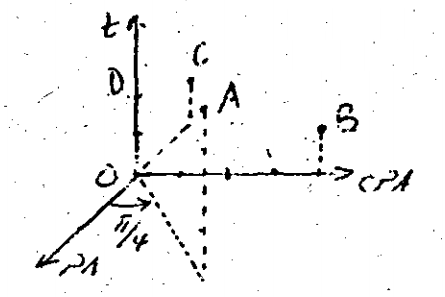
\includegraphics[width=0.3\textwidth]{images/b2p1-221-fig01}
	\\
\addtocounter{enumi}{1}
	\item ~\\
	 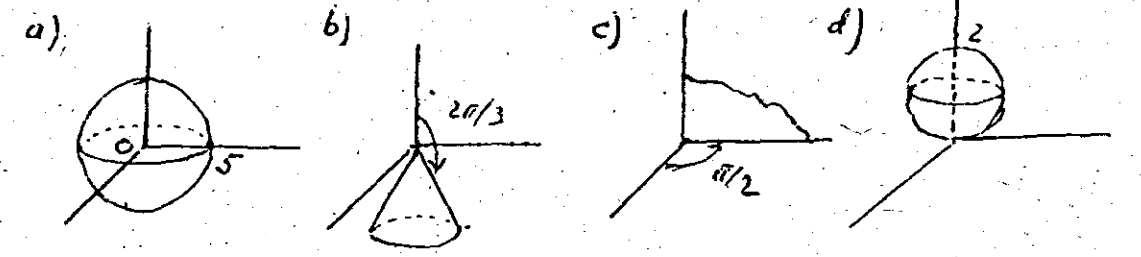
\includegraphics[width=0.9\textwidth]{images/b2p1-221-fig02}
	\\
\addtocounter{enumi}{1}
	\item ~\\
	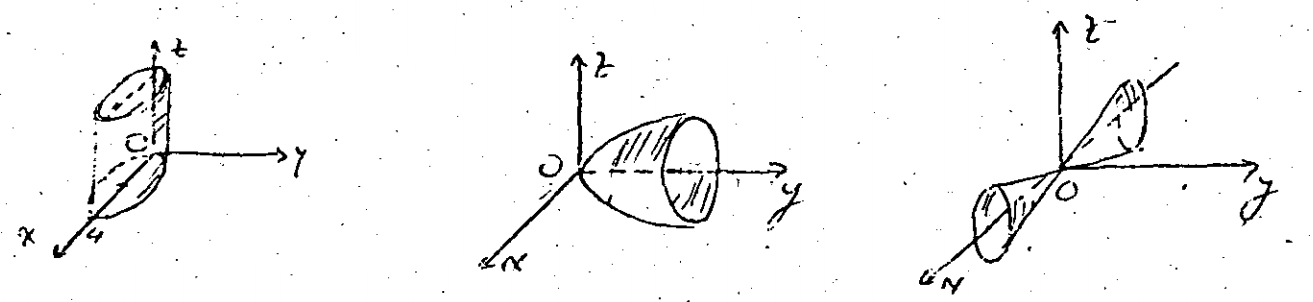
\includegraphics[width=0.9\textwidth]{images/b2p1-221-fig03}
	
\addtocounter{enumi}{1}
	\item 
		\begin{enumerate}[label=\alph*)]
			\begin{multicols}{2}	
				\item $2x+z^2=8$
				\item $y=(x-2)^2$
			\end{multicols}
		\end{enumerate}
	
\addtocounter{enumi}{1}
	\item 
		\begin{enumerate}[label=\alph*)]
			\begin{multicols}{3}	
				\item $y^2+z^2=3x-16$
				\item $x^2+y^2=2pz$
				\item $\frac{x^2}{a^2}-\frac{y^2}{b^2}+\frac{z^2}{a^2}=1$					
			\end{multicols}
		\end{enumerate}

\end{enumerate}


% =======================================================
\end{document}  

